\documentclass[aps,12pt,prd,nofootinbib,bibnotes, amsmath,amssymb,showpacs,superscriptaddress,floatfix]{revtex4-2}
\bibliographystyle{apsrev}
\usepackage[utf8]{inputenc}
\usepackage{epsf,epsfig,graphics}
\usepackage{graphicx,amsmath,mathrsfs,amssymb, amsthm,nccbbb,cancel,xcolor,wrapfig,siunitx,longtable,tabularx,CJKutf8,subfigure,float,xspace,physics,esvect,braket,enumitem,url,makeidx}
\usepackage{verbatim,color,ulem}
\usepackage{bm}
\usepackage[mathscr]{eucal}
\usepackage{hyperref}
\usepackage[toc,page]{appendix}
\usepackage[hang, flushmargin]{footmisc}
\usepackage{footnotebackref}

%%%%%%%%%%%%%%%%%%%%%%%%%%%%%%%%%%%%%%%%%%%
\begin{document}
\title{Computational Astrophysics HW3}
\author{Yi-Hsiang Kuo, 110022506}
\date{Oct. 27, 2022}
\maketitle
%\tableofcontents
%%%%%%%%%%%%%%%%%%%%%%%%%%%%%%%%%%%%%%%%%%%
\section{Exercise 2}
(1) The equation of {\bf{vector norm ($L_p$-norms)}}:
\begin{equation}
||x||_p = (\sum^n_{i = 1}|x_i|^p)^\frac{1}{p} 
\end{equation}

After calculation, we can get {\color{blue}{first and second norms $3.3$ and $2.7$ respectively}}

for {\bf{infinite norm}}, applying:
\begin{equation}
||x||_{\infty} = max|x_i|, \quad 1 \leq i \leq n
\end{equation}

and get the answer: {\color{blue}{2.6}}. \\
 
(2) For the matrix $A$, applying the {\bf{matrix norm}} formula:
\begin{equation}
||A|| = max_{x \neq 0} \frac{||Ax||}{||x||}
\end{equation}
\begin{equation}
||A||_1 = max_j \sum_{i=1}^n |a_{ij}|
\end{equation}
\begin{equation}
||A||_{\infty} = max_i \sum_{j=1}^n |a_{ij}|
\end{equation}

we can get the {\color{blue}{L1-norm (maximum absolute column sum):78}}, and the {\color{blue}{$L_{\infty}$-norm (maximum absolute row sum):83}} \\

\section{Exercise 3}
To evaluate the real root(s) of:
\begin{equation}
x^3+1.5 x^2 -5.75 x +4.37 = 0
\end{equation}

using {\color{blue}{(a) bisection method}} with initial guess from $-4.0$ to $-3.0$; {\color{blue}{(b) Newton-Raphson's method}} with initial point $x=-3.0$ and {\color{blue}{(c) secant method}} with initial guess from $-4.0$ to $-3.0$, and FIG. 1. is the comparison result.
\begin{figure}
	\centering
	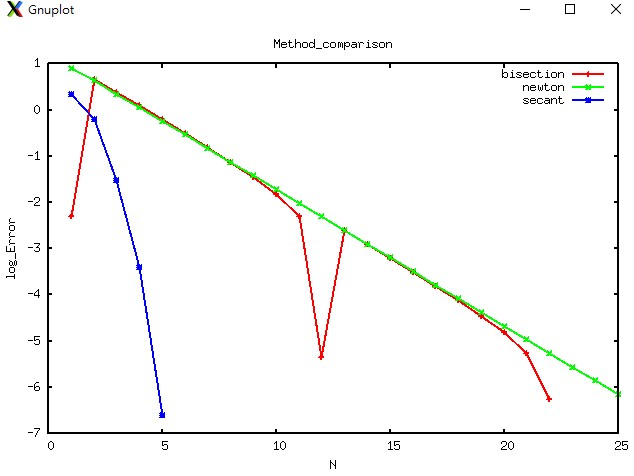
\includegraphics[width=1.0\textwidth]{EX3_Method_comparison}
	\caption{Exercise3 Method comparison}
\end{figure}

By the way, for {\color{blue}{Newton-Raphson's method}}, if our initial guess is $x=-3.5$, the iteration value N still need to approach $N=14$, it seems that {\color{blue}{(c) secant method}} is the best way here.   
    
\section{Exercise 4}
(1)(2)(3) The analytical calculations wrote on FIG. 2. : 
\begin{figure}
	\centering
	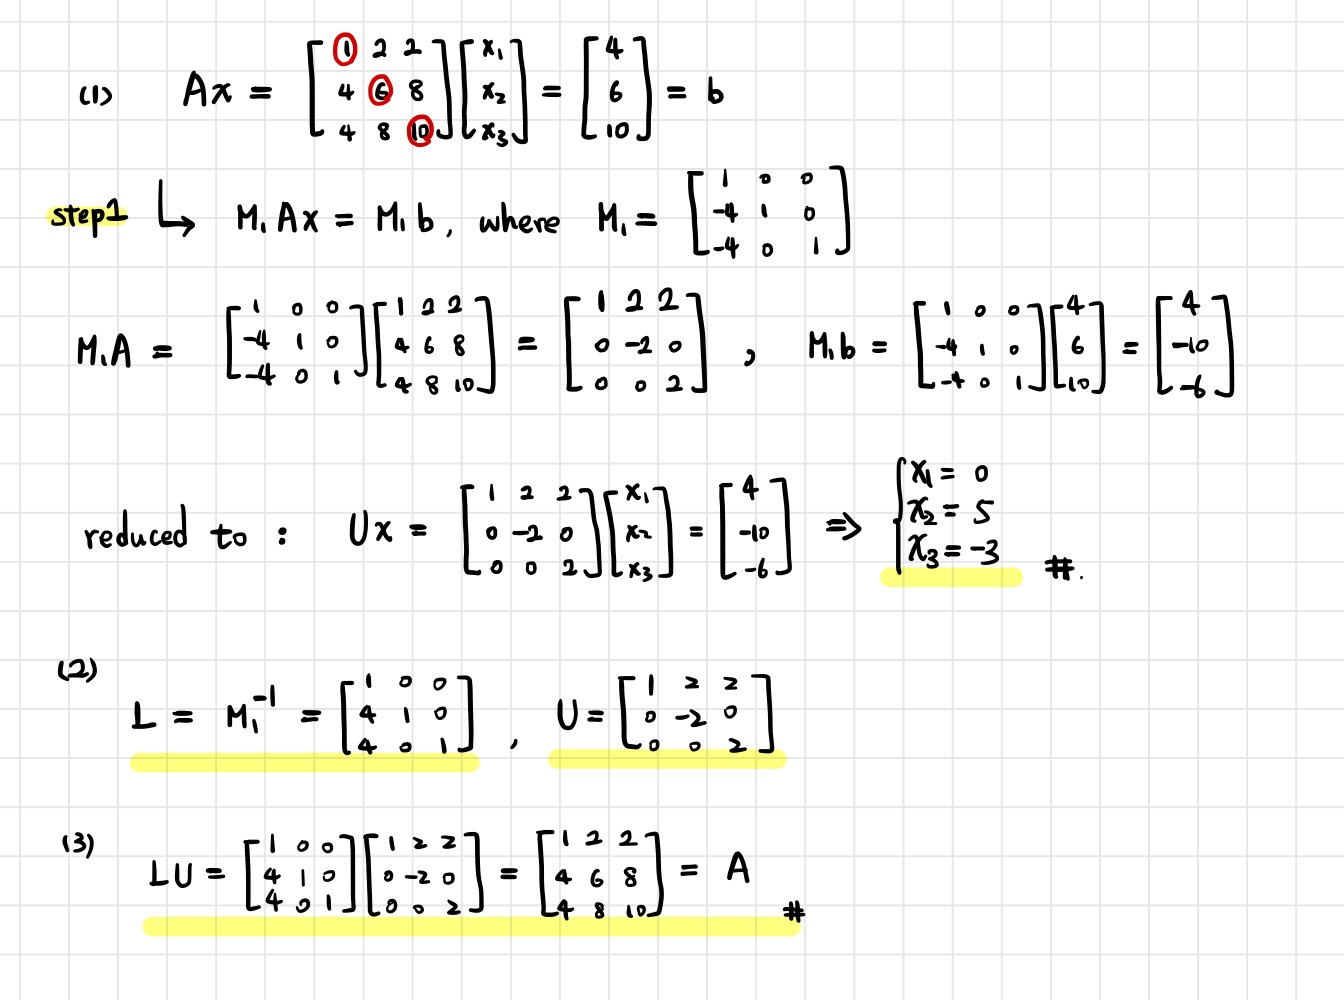
\includegraphics[width=1.0\textwidth]{EX4}
	\caption{Exercise4 Gaussian elimination}
\end{figure}



\section{Exercise 5}
(1)(2)(3) I have finished the subroutine $LU \_ decomposition$ in $linalg.f90$ and the  \href{https://github.com/kuo1235/Computational-Astrophysics-2022/blob/main/astr660/week6/exercise/L6exercise/linalg.f90}{\bf{git gub link is here}}, put two different matrix $A$ from in-class exercise and Exercise 4, the result is the following figures: 
\begin{figure}[htbp]
\centering
\begin{minipage}[t]{0.48\textwidth}
\centering
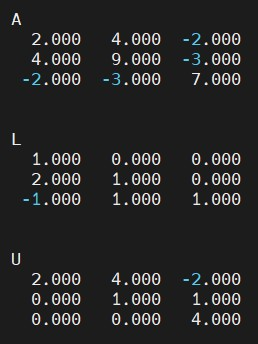
\includegraphics[width=6cm]{EX5_1}
\caption{Ex5-1 result}
\end{minipage}
\begin{minipage}[t]{0.48\textwidth}
\centering
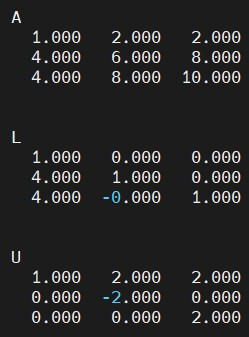
\includegraphics[width=6cm]{EX5_2}
\caption{Ex5-2 result}
\end{minipage}
\end{figure}

Next, further call $solve \_ lower \& upper \_ triangular \_ matrix$, we can get the soltion $x$ as the following figure, and the result indeed meets my answer in Exercise 4.

\begin{figure}
	\centering
	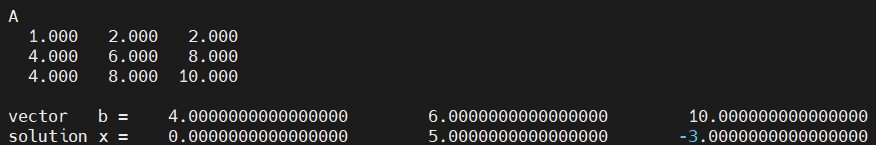
\includegraphics[width=1.0\textwidth]{EX5_3}
	\caption{Ex5-3 result}
\end{figure}
\section{Exercise 6}
(1) I build up the code $Ex6 \_ 1$ \href{https://github.com/kuo1235/Computational-Astrophysics-2022/blob/main/astr660/Homework/HW3/EX6/EX6_1.py}{\bf{link here}} to build up matrix $A$ and using $linalg \_ lu.solve$ to get the value x, see FIG. 6. 
\begin{figure}
	\centering
	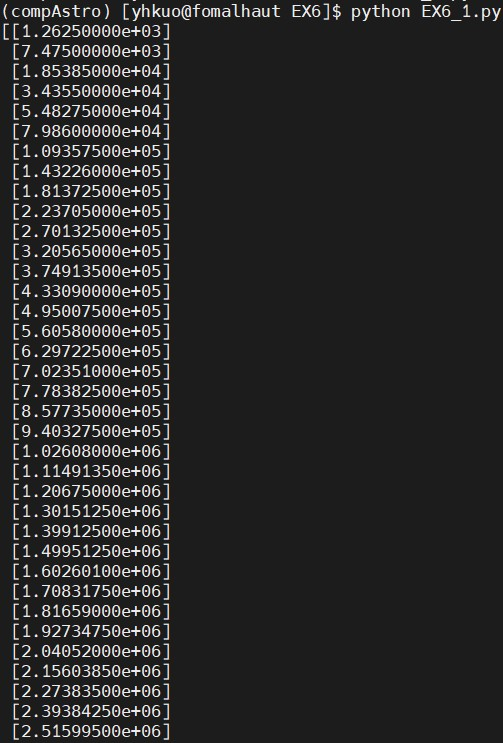
\includegraphics[width=1.0\textwidth]{EX6_1}
	\caption{Ex6-1 (a portion of) x}
\end{figure}

(2) using another method $scipy.linalg.solve_banded$ and the code $Ex6 \_ 2$ \href{https://github.com/kuo1235/Computational-Astrophysics-2022/blob/main/astr660/Homework/HW3/EX6/EX6_2.py}{\bf{link here}}, we can get same $x$ as from Ex6-1.

For the computing time, I use $timeit$ as my tool monitoring the running time and FIG. 7. is the result. LU decomposition costs about $1.74ms$, and bandmatrix method cost only about $542 \mu s$ 
\begin{figure}
	\centering
	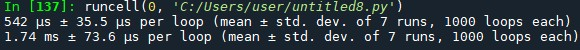
\includegraphics[width=1.0\textwidth]{EX6_2}
	\caption{Ex6-2 Computing time}
\end{figure}


(3)By using $np.linalg.cond$, the condition number of matrix A is about $130661079.52047908$ 


\bibliographystyle{apsrev}
\bibliography{Ref}
\end{document}







